\chapter{Linux Commands \\
\small{\textit{-- Tamara Gonzalez Ibarra, Michelle Elias Flores, Sydney Winstead}}
\index{itLinuxCommands} 
\index{Chapter!itLinuxCommands}
\label{Chapter::itLinuxCommands}}

In this chapter, we have included the following screenshots of our work for the Linux Commands assignment. Completing this assignment involved practicing Linux commands for navigation, file operations, permissions, process control, networking, and scripting. 

\begin{figure}[h!]
    \centering
    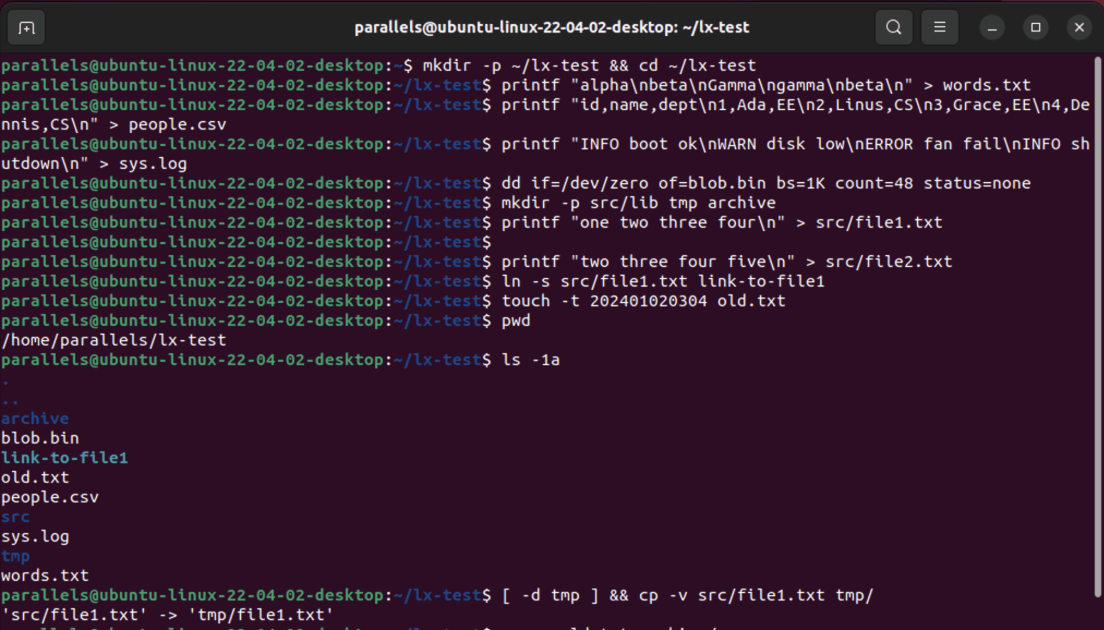
\includegraphics[width=0.8\textwidth]{linuxptA.png}
    \caption{Screenshot of the first part of A) Navigation and File Operations}
    \label{fig:problemsetA}
\end{figure}
    
\begin{figure}[h!]
    \centering
    
\includegraphics[width=0.8\textwidth]{linuxptA2.png}
    \caption{Screenshot of the second part of A) Navigation and File Operations}
    \label{fig:problemsetApt2}
\end{figure}

\begin{figure}[h!]
    \centering
    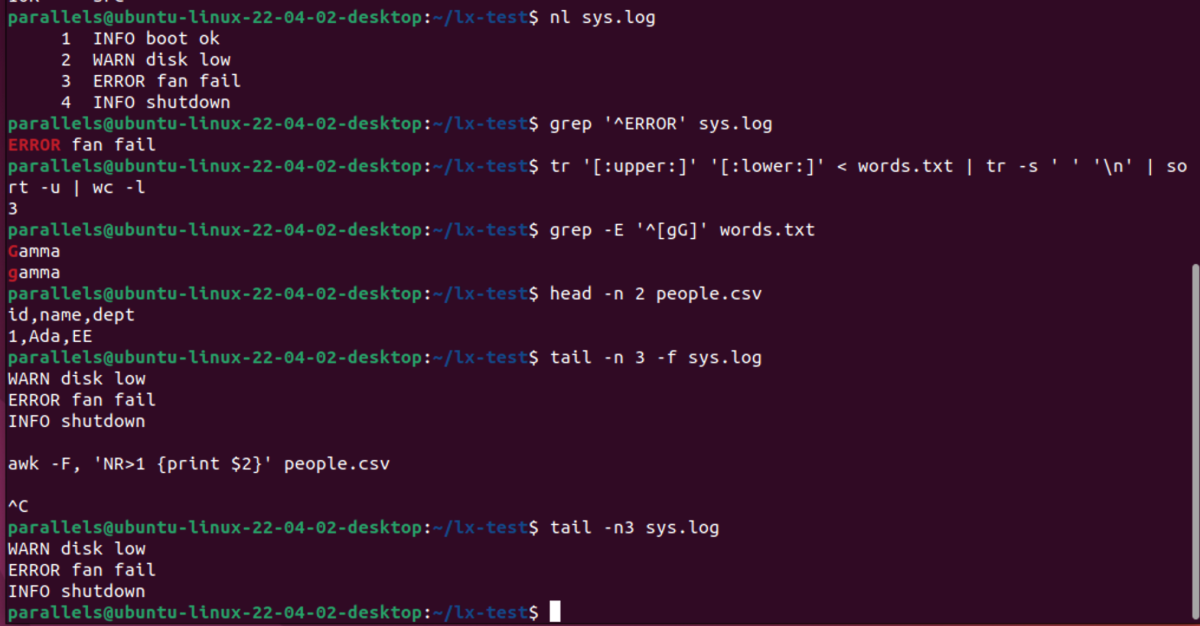
\includegraphics[width=0.8\textwidth]{linuxptB.png}
    \caption{Screenshot of Part B) Viewing and Searching}
    \label{fig:problemsetB}
\end{figure}

\begin{figure}[h!]
    \centering
    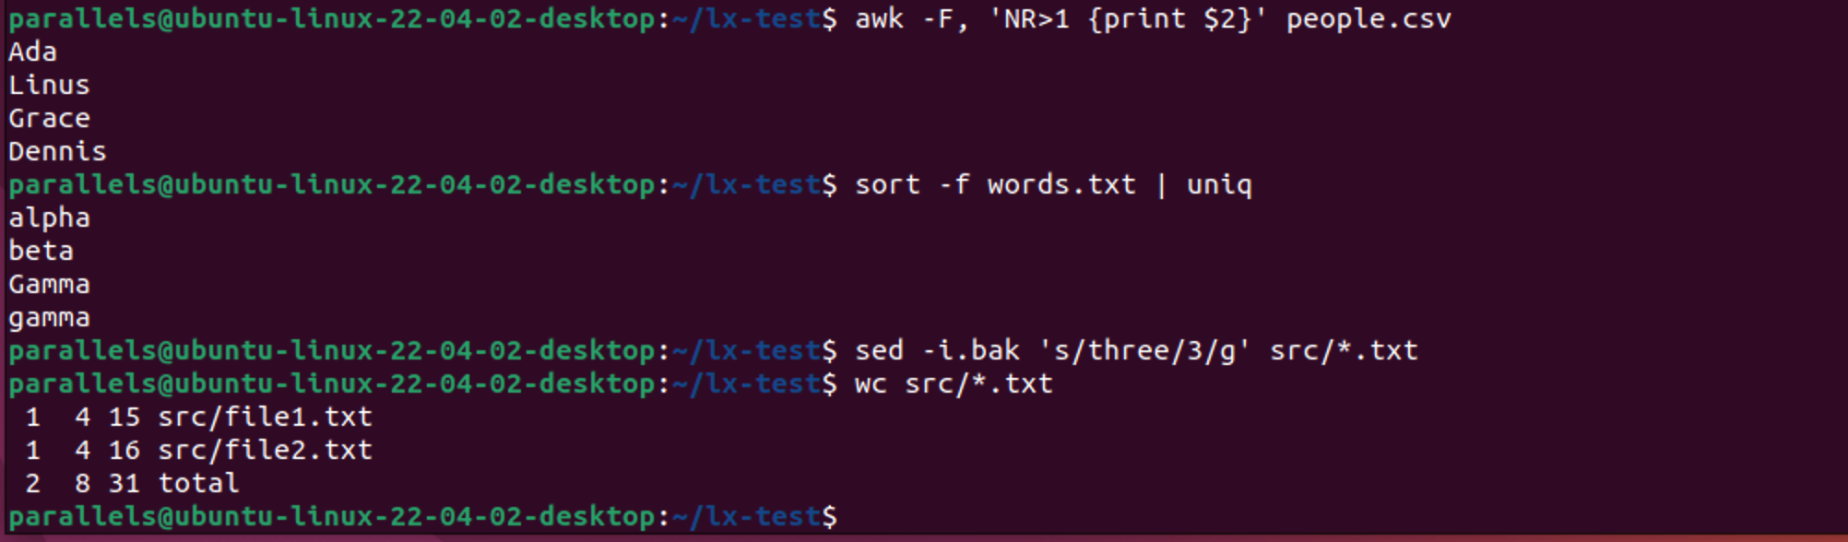
\includegraphics[width=0.8\textwidth]{linuxptC.png}
    \caption{Screenshot of Part C) Text Processing}
    \label{fig:problemsetC}
\end{figure}

\begin{figure}[h!]
    \centering
    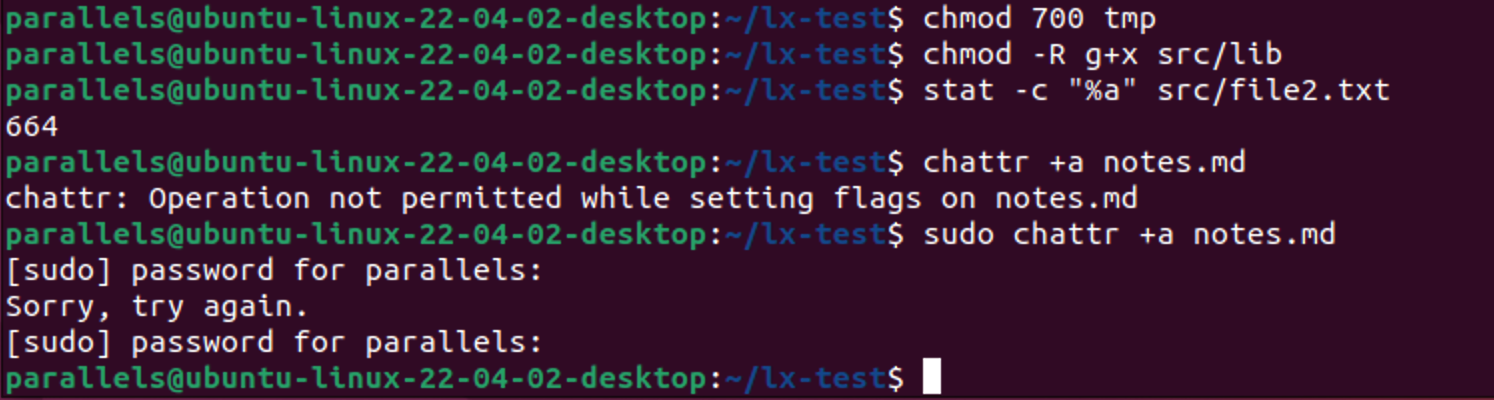
\includegraphics[width=0.8\textwidth]{linuxptD.png}
    \caption{Screenshot of Part D) Permissions and Ownership}
    \label{fig:problemsetD}
\end{figure}

\begin{figure}[h!]
    \centering
    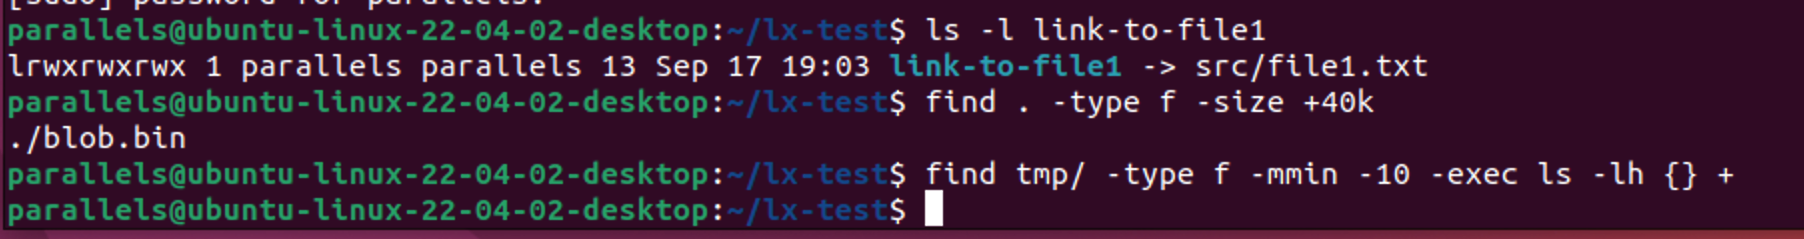
\includegraphics[width=0.8\textwidth]{linuxptE.png}
    \caption{Screenshot of Part E) Links and Find}
    \label{fig:problemsetE}
\end{figure}

\begin{figure}[h!]
    \centering
    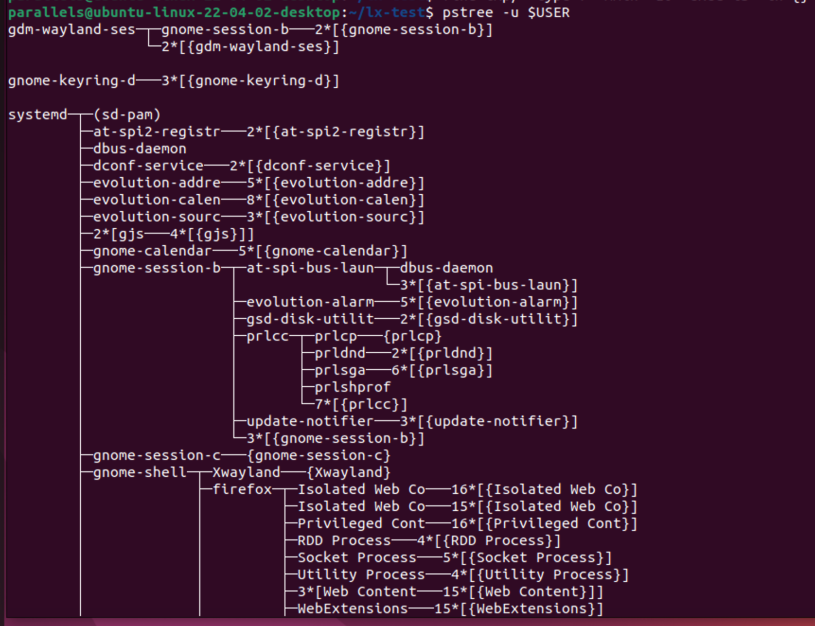
\includegraphics[width=0.8\textwidth]{linuxptF.png}
    \caption{Screenshot of the first part of Part F) Processes and Job Control}
    \label{fig:problemsetF}
\end{figure}

\begin{figure}[h!]
    \centering
    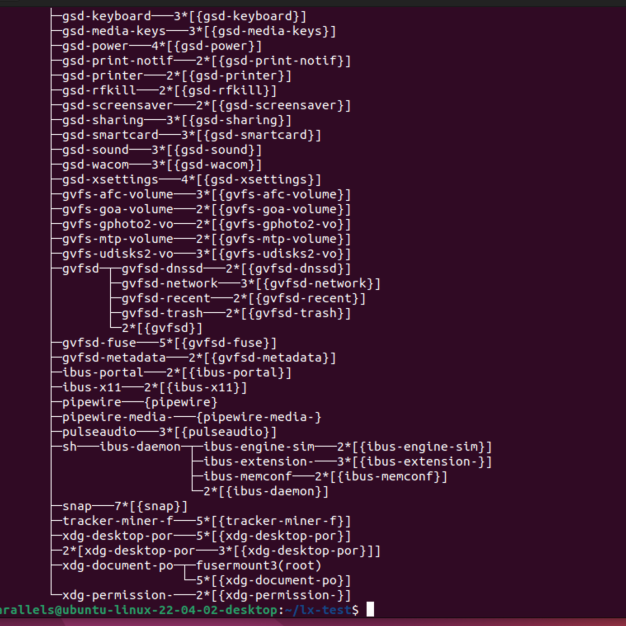
\includegraphics[width=0.8\textwidth]{linuxptF2.png}
    \caption{Screenshot of the second part of Part F) Processes and Job Control}
    \label{fig:problemsetFpt2} % fixed label
\end{figure}

\begin{figure}[h!]
    \centering
    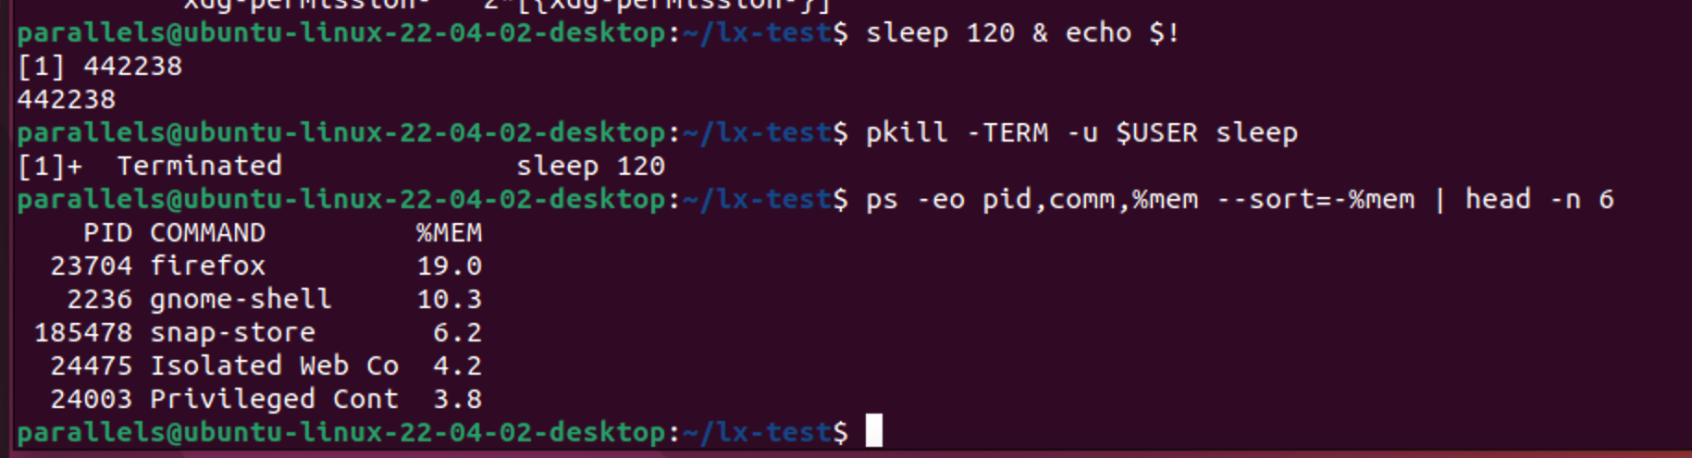
\includegraphics[width=0.8\textwidth]{linuxptF3.png}
    \caption{Screenshot of the third part of Part F) Processes and Job Control}
    \label{fig:problemsetFpt3}
\end{figure}

\begin{figure}[h!]
    \centering
    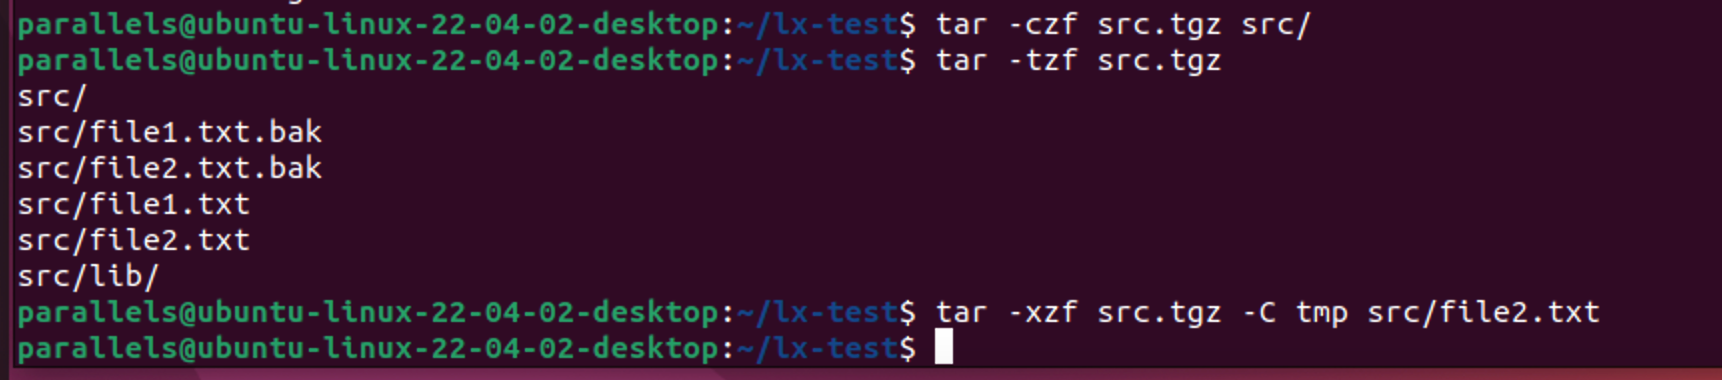
\includegraphics[width=0.8\textwidth]{linuxptG.png}
    \caption{Screenshot of Part G) Archiving and Compression}
    \label{fig:problemsetG}
\end{figure}

\begin{figure}[h!]
    \centering
    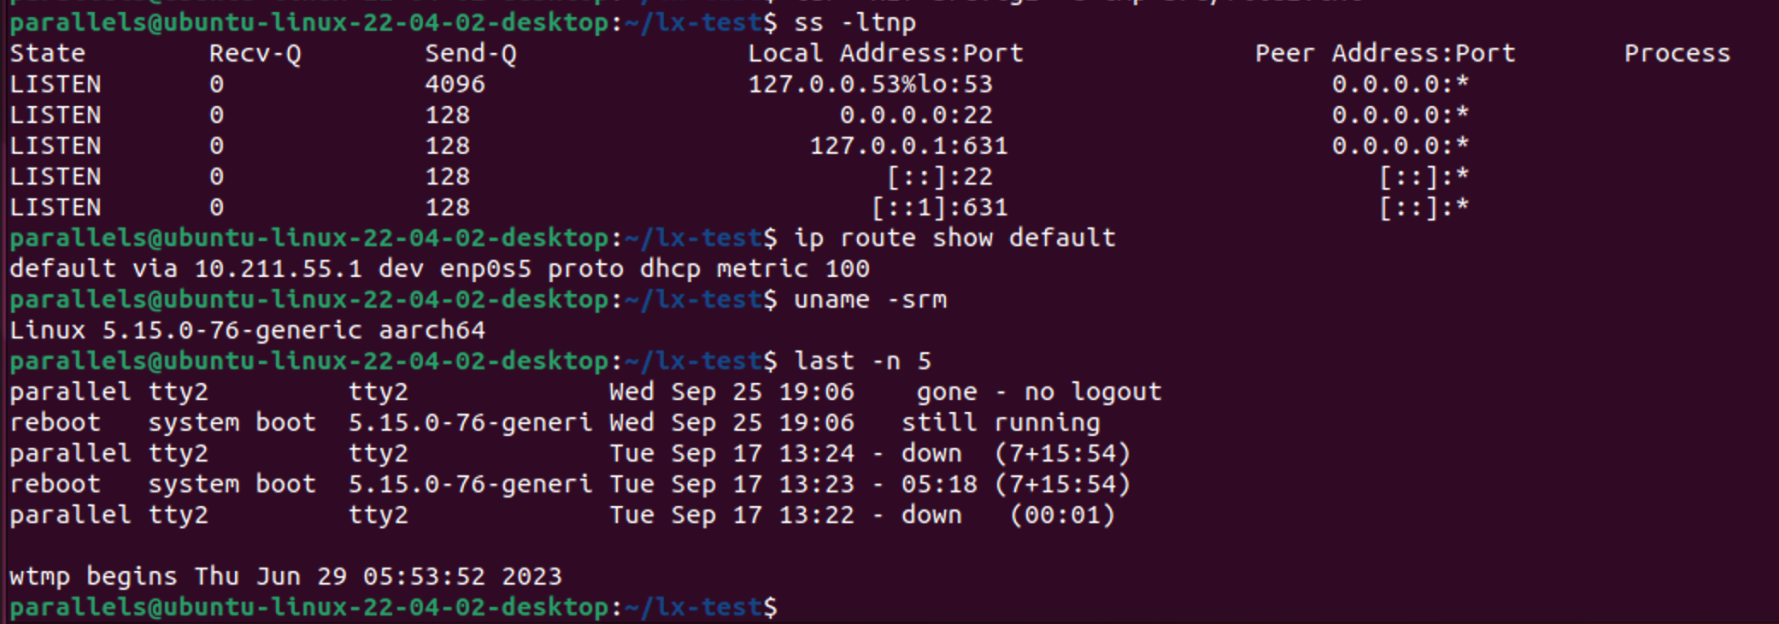
\includegraphics[width=0.8\textwidth]{linuxptH.png}
    \caption{Screenshot of Part H) Networking and System Information}
    \label{fig:problemsetH}
\end{figure}

\begin{figure}[h!]
    \centering
    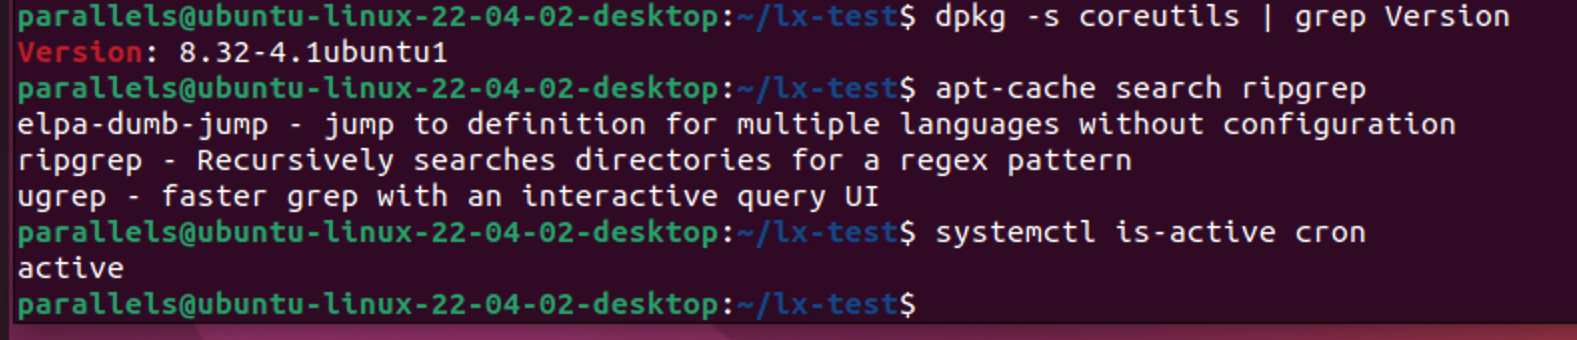
\includegraphics[width=0.8\textwidth]{linuxptI.png}
    \caption{Screenshot of Part I) Package and Services (Debian/Ubuntu)}
    \label{fig:problemsetI}
\end{figure}

\begin{figure}[h!]
    \centering
    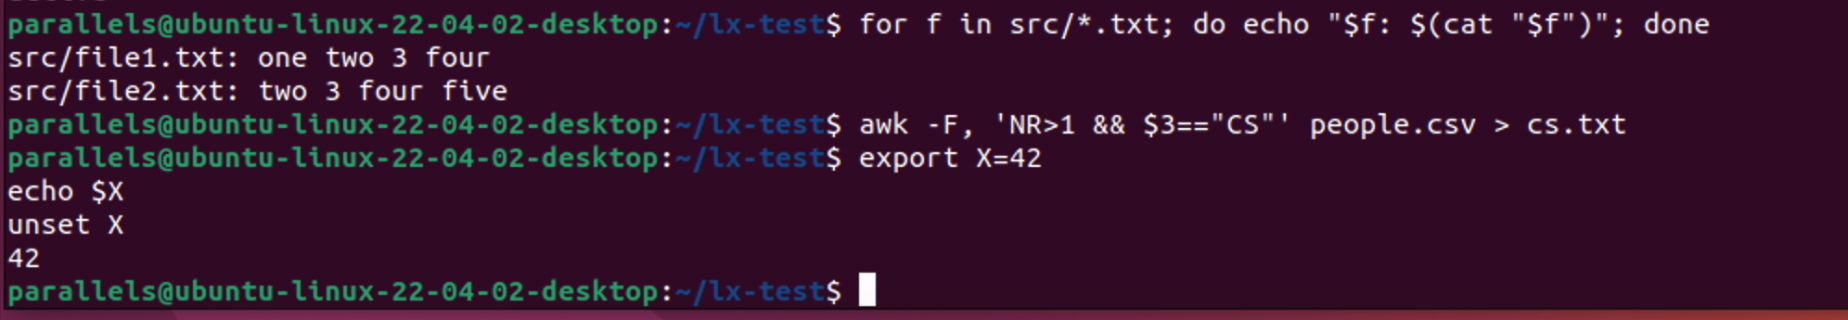
\includegraphics[width=0.8\textwidth]{linuxptJ.png}
    \caption{Screenshot of Part J) Bash and Scripting}
    \label{fig:problemsetJ}
\end{figure}
